%\documentclass[letterpaper,11pt]{article}
\documentclass[letterpaper,11pt,twocolumn]{article}
\usepackage{graphics,graphicx}
\setlength{\textwidth}{6.5in} \setlength{\textheight}{9in}
\setlength{\topmargin}{-0.0625in} \setlength{\oddsidemargin}{0in}
\setlength{\evensidemargin}{0in} \setlength{\headheight}{0in}
\setlength{\headsep}{0in} \setlength{\hoffset}{0in}
\setlength{\voffset}{0in}

\makeatletter
\renewcommand{\section}{\@startsection%
{section}{1}{0mm}{-\baselineskip}%
{0.5\baselineskip}{\normalfont\Large\bfseries}}%
\makeatother

\begin{document}
\pagestyle{plain}
\pagenumbering{arabic}

\begin{center} 
\bfseries\uppercase{%
The Candidate LLAGN in the Nearby Elliptical Galaxy NGC\,4621
}
\end{center}

\section{Scientific Justification}

A133, detected at 1.4 in all configs
A539, no 1.4 in C, no 4.89 in B
A1204, detected at 1.4 in B but not C
A2107, detected at 1.4 in B
A2556, detected at 1.5 in B/C
AWM7, no 1.4 in A or B
ESO 5520200, unobserved
MKW4, detected at 1.4 in B
MS J0440.5+0204, detected at 1.4, cool double src
MS J1159.8+5531, detected at 1.4 in B

\section{Technical Justification}

%% \begin{figure}[tbh]
%% \includegraphics[scale=0.4]{f1.eps}
%% \caption{\em{NGC\,4621 at 0.5-8 keV over a field of view of 90 arcsec.
%% The strongest source is the candidate nucleus and has $L(2-10~keV) =
%% 6.8 \times 10^{37}$~ergs~s$^{-1}$. 1 arcsec = 88~pc.}}
%% \end{figure}

\section{References}

\end{document}
